\documentclass[border={0.1cm 0.1cm 0.1cm 0.1cm}]{standalone}  %E,S,W,N

\usepackage{amssymb}
\usepackage{amsmath}
\usepackage{tikz}
\usetikzlibrary{shapes} %for node shapes
\usetikzlibrary{calc}	%for centerarc

%NOTE: MODIFIED DEFINITION OF CENTERARC
\def\centerarc[#1](#2)(#3:#4:#5) {\draw[#1] ($(#2)+({#5*cos(#3)},{#5*sin(#3)})$) arc (#3:#4:#5)}

%HOW TO READ (guessing):
%The rightmost circle is the sun; the 0-degree circle is the moon
%The other circles are the earth; note the red inner part facing the moon
%The original has inconsistencies: color for 90-degree circle + reversed red part for 50-degrees

\begin{document}
	
	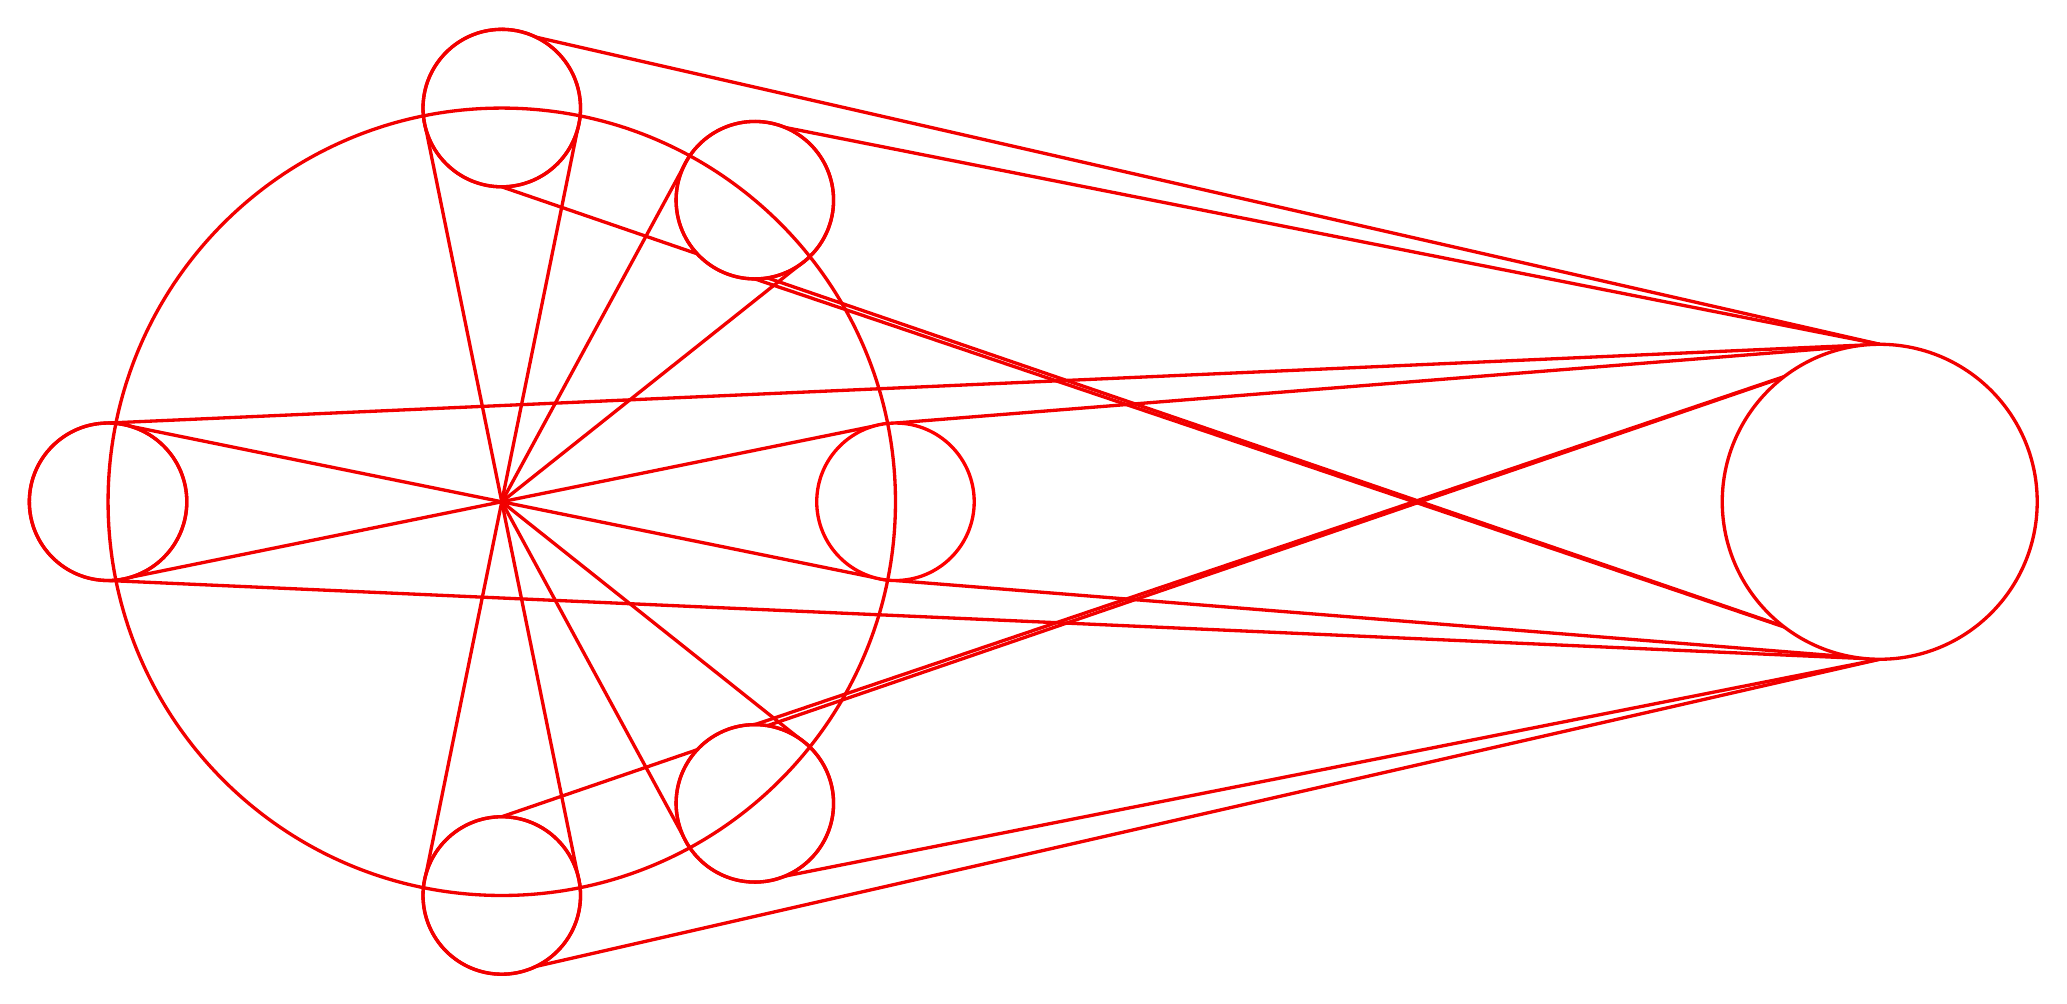
\begin{tikzpicture}[very thick,red!95!black]
	\foreach \i in {0,90,-90,50,-50,180}{
		\draw ({5*cos(\i)},{5*sin(\i)+1}) -- ({17.5+2*cos(90)},{2*sin(90)});
		\draw ({5*cos(\i)},{5*sin(\i)-1}) -- ({17.5+2*cos(-90)},{2*sin(-90)});
		\draw (0,0) -- ({5*cos(\i+11.5)},{5*sin(\i+11.5)});
		\draw (0,0) -- ({5*cos(\i-11.5)},{5*sin(\i-11.5)});
		\filldraw[very thick,draw=red,fill=white] ({5*cos(\i)},{5*sin(\i)}) circle (1cm);
		%\centerarc[fill=black](0,0)(\i+11.5:\i-11.5:5) arc ({\i-90-5}:\i+90+5:1);
		%\draw ({5*cos(\i)},{5*sin(\i)}) circle (1cm);
	}
	
	%SHADING OUTER CIRCLE
	\foreach \i in {90,-90,50,-50,180}{
		\centerarc[fill=black](0,0)(\i+11.5:\i-11.5:5) arc ({\i-90-5}:{\i+90+5}:1);
		\draw ({5*cos(\i)},{5*sin(\i)}) circle (1cm);
	}
	
	%SHADING INNER CIRCLE
	\centerarc[fill=black](0,0)(0-11.5:0+11.5:5) arc (95:95+170:1); %0
	\centerarc[fill=red!95!black,draw=red!95!black](0,0)(180-11.5:180+11.5:5) arc (180+90+5:180+90+170:1); %180
	
	%PARTIAL INNER SHADING
	\centerarc[fill=red!95!black](0,0)(50-11.5:50:5) -- ({5*cos(50)+cos(50+180)},{5*sin(50)+sin(50+180)}) arc ({50+180}:{50+180+2*50}:1);
	\centerarc[fill=red!95!black](0,0)(90-11.5:90:5) -- ({5*cos(90)+cos(90+180)},{5*sin(90)+sin(90+180)}) arc ({90+180}:{90+180+90}:1);
	\centerarc[fill=red!95!black](0,0)(-90+11.5:-90:5) -- ({5*cos(-90)+cos(-90+180)},{5*sin(-90)+sin(-90+180)}) arc ({-90+180}:{-90+180-90}:1);
	%\centerarc[fill=red!95!black](0,0)(-50-11.5:-50:5) -- ({5*cos(-50)+cos(-50+180)},{5*sin(-50)+sin(-50+180)}) arc ({-50+180}:{-50+180+60}:1); %original
	\centerarc[fill=red!95!black](0,0)(-50+11.5:-50:5) -- ({5*cos(-50)+cos(-50+180)},{5*sin(-50)+sin(-50+180)}) arc ({-50+180}:{-50+180-60}:1);
	
	\draw (0,0) circle (5cm);
	\filldraw[very thick,draw=red!95!black,fill=white] (17.5,0) circle (2cm);
	\end{tikzpicture}
	
\end{document}